\section{Gemmini Evaluation}\label{sec:evaluation}
This section discusses our evaluation methodology and evaluation results of Gemmini-generated accelerators compared to both CPUs and state-of-the-art, commercial accelerators.

\subsection{Evaluation Methodology}

We evaluate the end-to-end performance of Gemmini-generated accelerators using the FireSim FPGA-accelerated simulation platform~\cite{karandikar2018firesim}. We evaluate five popular DNNs: ResNet50, AlexNet, SqueezeNet v1.1, MobileNetV2, and BERT.
All DNNs are evaluated with a full Linux environment on a complete cycle-exact simulated SoC.
We synthesize designs using Cadence Genus with the Intel 22nm FFL process technology and place-and-route them using Cadence Innovus.
Our layout and area breakdown, described in Figure~\ref{fig:evaluation}, show that the SRAMs alone consume 67.1\% of the accelerator's total area. The spatial array itself only consumes 11.3\%, while the host CPU consumed a higher 16.6\% of area.

% We evaluated the end-to-end execution performance of Gemmini-generated accelerators on five commonly-used DNN workloads: ResNet50, AlexNet, SqueezeNet v1.1, MobileNetV2, and BERT.
% All the DNNs were evaluated with a full Linux environment on a complete cycle-exact simulated SoC, using the FireSim FPGA-accelerated simulation platform~\cite{karandikar2018firesim}.
% Additionally, for our physical design, we synthesized accelerators using Cadence Genus with the Intel 22nm FFL process technology and placed-and-routed them using Cadence Innovus.
% Our layout is illustrated in Figure~\ref{fig:area-layout}, and our area breakdown, described in Figure~\ref{tab:area-table}, shows that the SRAM memories alone consumed 67.1\% of the accelerator's total area. The spatial array itself only consumed 11.3\%, while the host CPU consumed a higher 16.6\% of area.

\subsection{Performance Results}

We evaluated the performance of several Gemmini configurations, with different host CPUs and different ``optional'' compute blocks, to determine how the accelerator and host CPU configuration may interact to impact end-to-end performance. In particular, we evaluated two host CPUs: a low-power in-order Rocket core, and a high-performance out-of-order BOOM core. We used two different Gemmini configurations:
one \textit{without} an optional im2col block, and the other \textit{with} an im2col block which allowed the accelerator to perform im2col on-the-fly, relieving the host CPU of that burden.

As illustrated in Figure~\ref{fig:perf-dnn}, when the accelerator is built without an on-the-fly im2col unit, its performance depends heavily on the host-CPU which becomes responsible for performing im2col during CNN inference.
A larger out-of-order BOOM host CPU increases performance by 2.0x across all CNNs.
The less complex the DNN accelerator is, the more the computational burden is shifted onto the CPU, giving the host CPU a larger impact on end-to-end performance.

\begin{figure}[t]
% \centering
\begin{subfigure}[b]{0.5\linewidth}
\centering
\scalebox{0.8} {
\begin{tabular}{ l | r | r }
\hline
\textbf{Component size} &  \textbf{\makecell{Area\\($\mu m ^2$)}} & \textbf{\makecell{\% of \\System\\Area}} \\
\hline
\hline
Spatial Array (16x16) & 116K & 11.3\% \\
Scratchpad (256 KB) & 544K & 52.9\%  \\
Accumulator (64 KB) & 146K & 14.2\%  \\
% Gemmini Control & 51K & 3.1\% \\
% \hline
% Total (Gemmini) & 858K & 52.5\% \\
% \hline
CPU (Rocket, 1 core) & 171K & 16.6\% \\
% Shared L2 (512 KB) &  534K & 32.7\%  \\
% Buses and Peripherals & 70K & 4.3\%  \\
\hline
% Total (Overall) & 1,632K & 100.0\% \\
Total & 1,029K & 100.0\% \\
\hline
\end{tabular}
}
\caption{Area breakdown.}
\label{tab:area-table}
\end{subfigure}
\hfill
\begin{subfigure}[b]{0.4\linewidth}
\centering
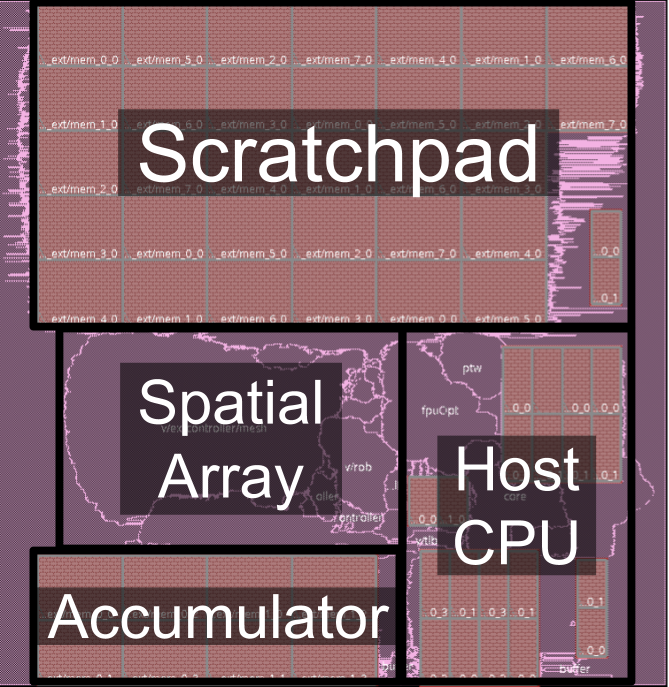
\includegraphics[width=0.8\linewidth]{fig/pnr.png}
\caption{Layout.}
\label{fig:area-layout}
\end{subfigure}
% \begin{subfigure}[b]{0.45\linewidth}
% \centering
% 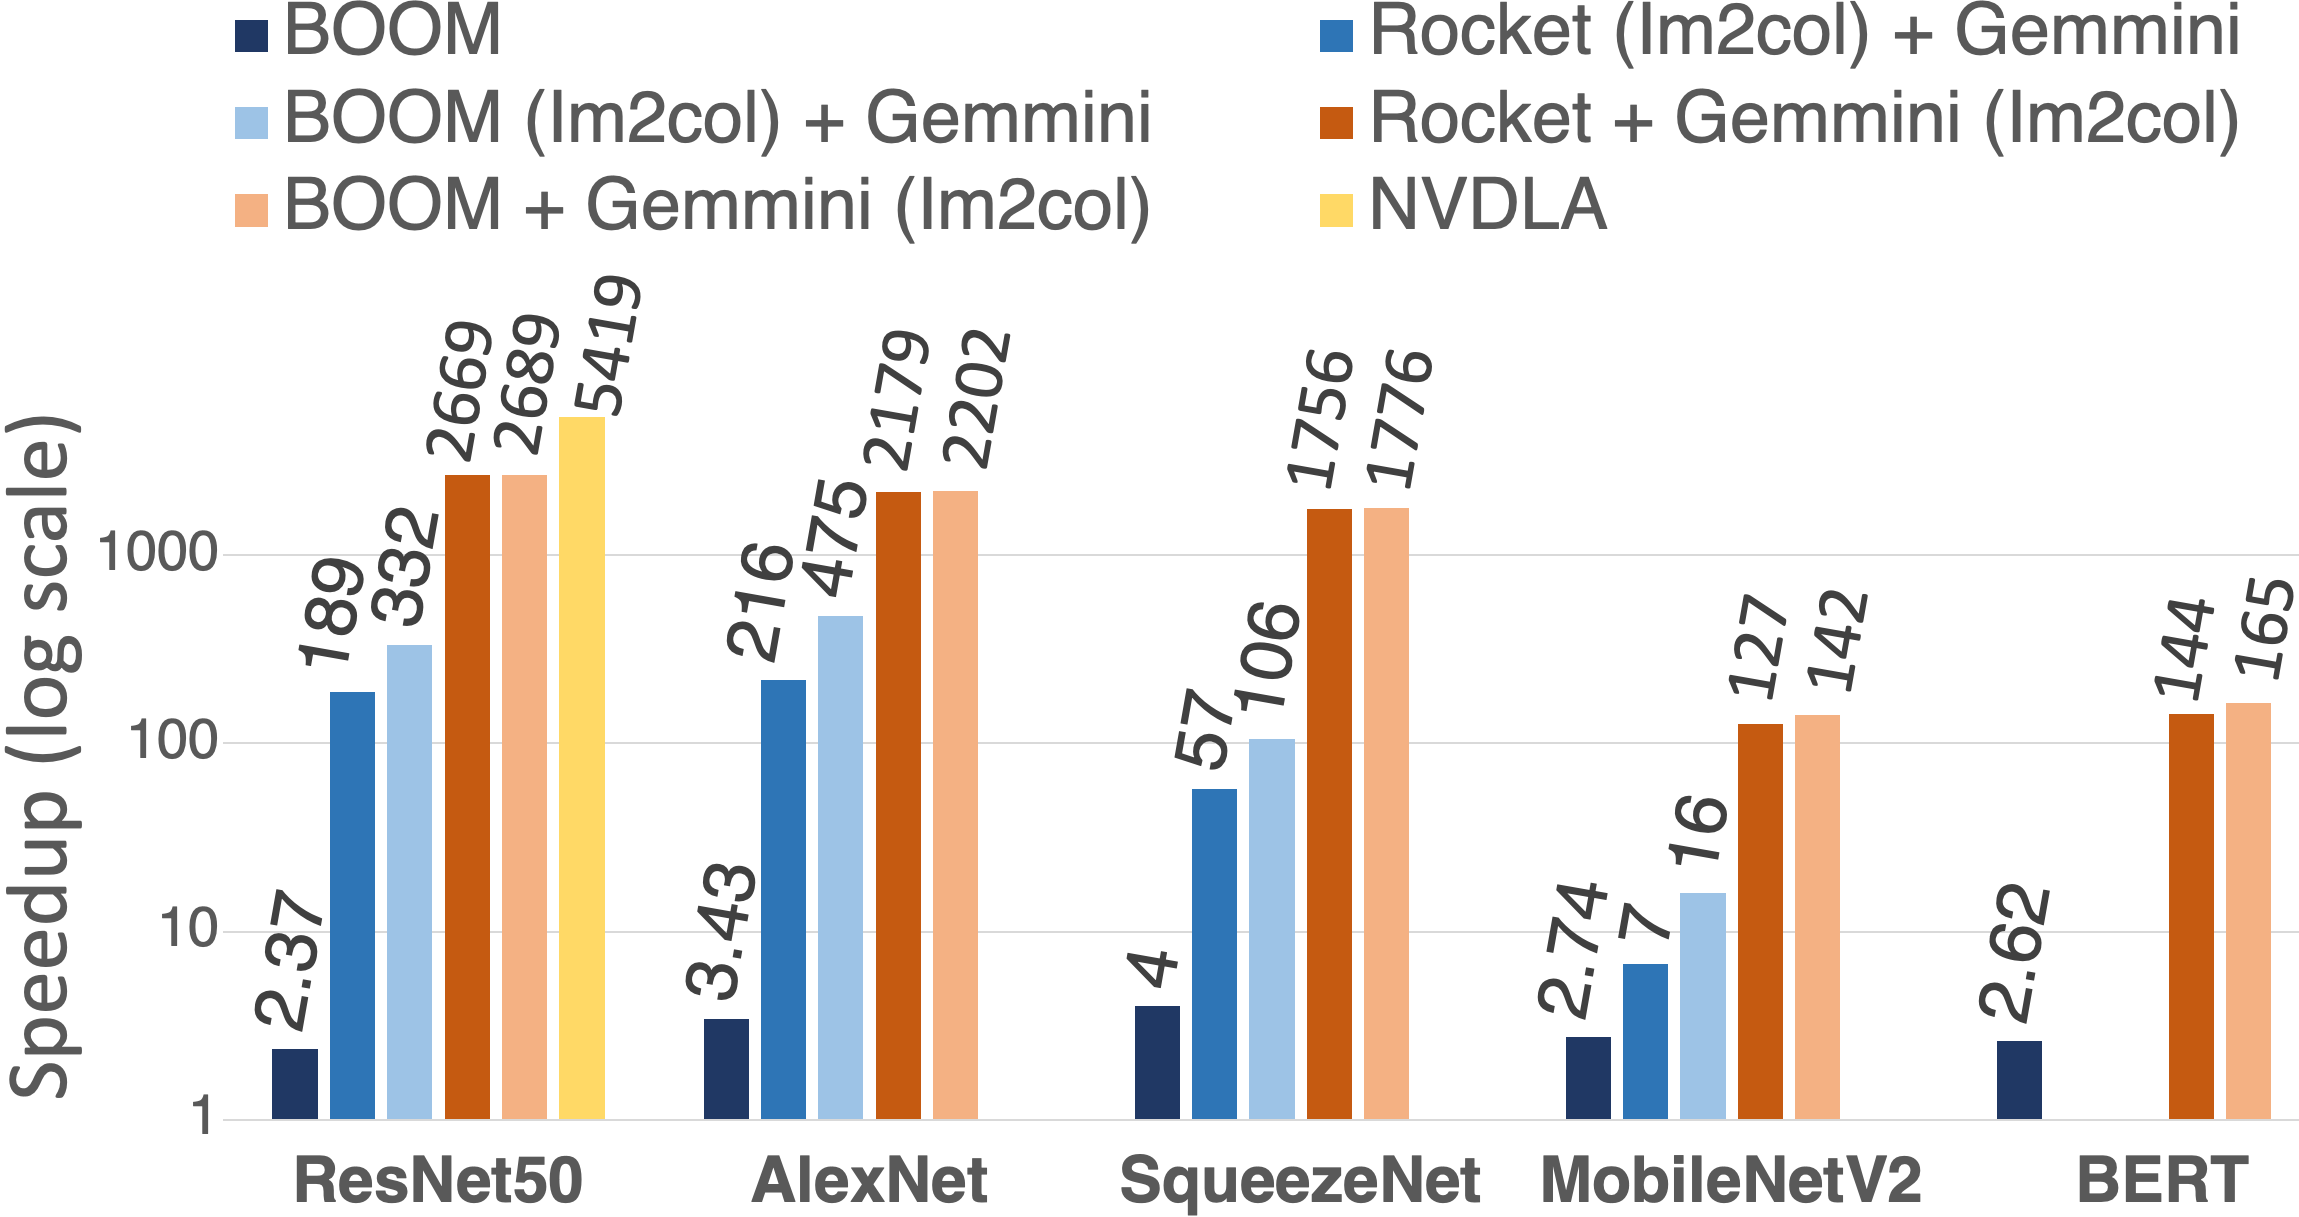
\includegraphics[width=\linewidth]{fig/perf-conv-new.png}
% \caption{Performance compared to an in-order CPU baseline. For CNNs, im2col was performed on either the CPU, or on the accelerator.}
% \label{fig:perf-dnn}
% \end{subfigure}
\caption{Area breakdown and layout of accelerator with host CPU.}
\label{fig:evaluation}
\vspace{-0.2in}
\end{figure}

\begin{figure}[b]
\centering
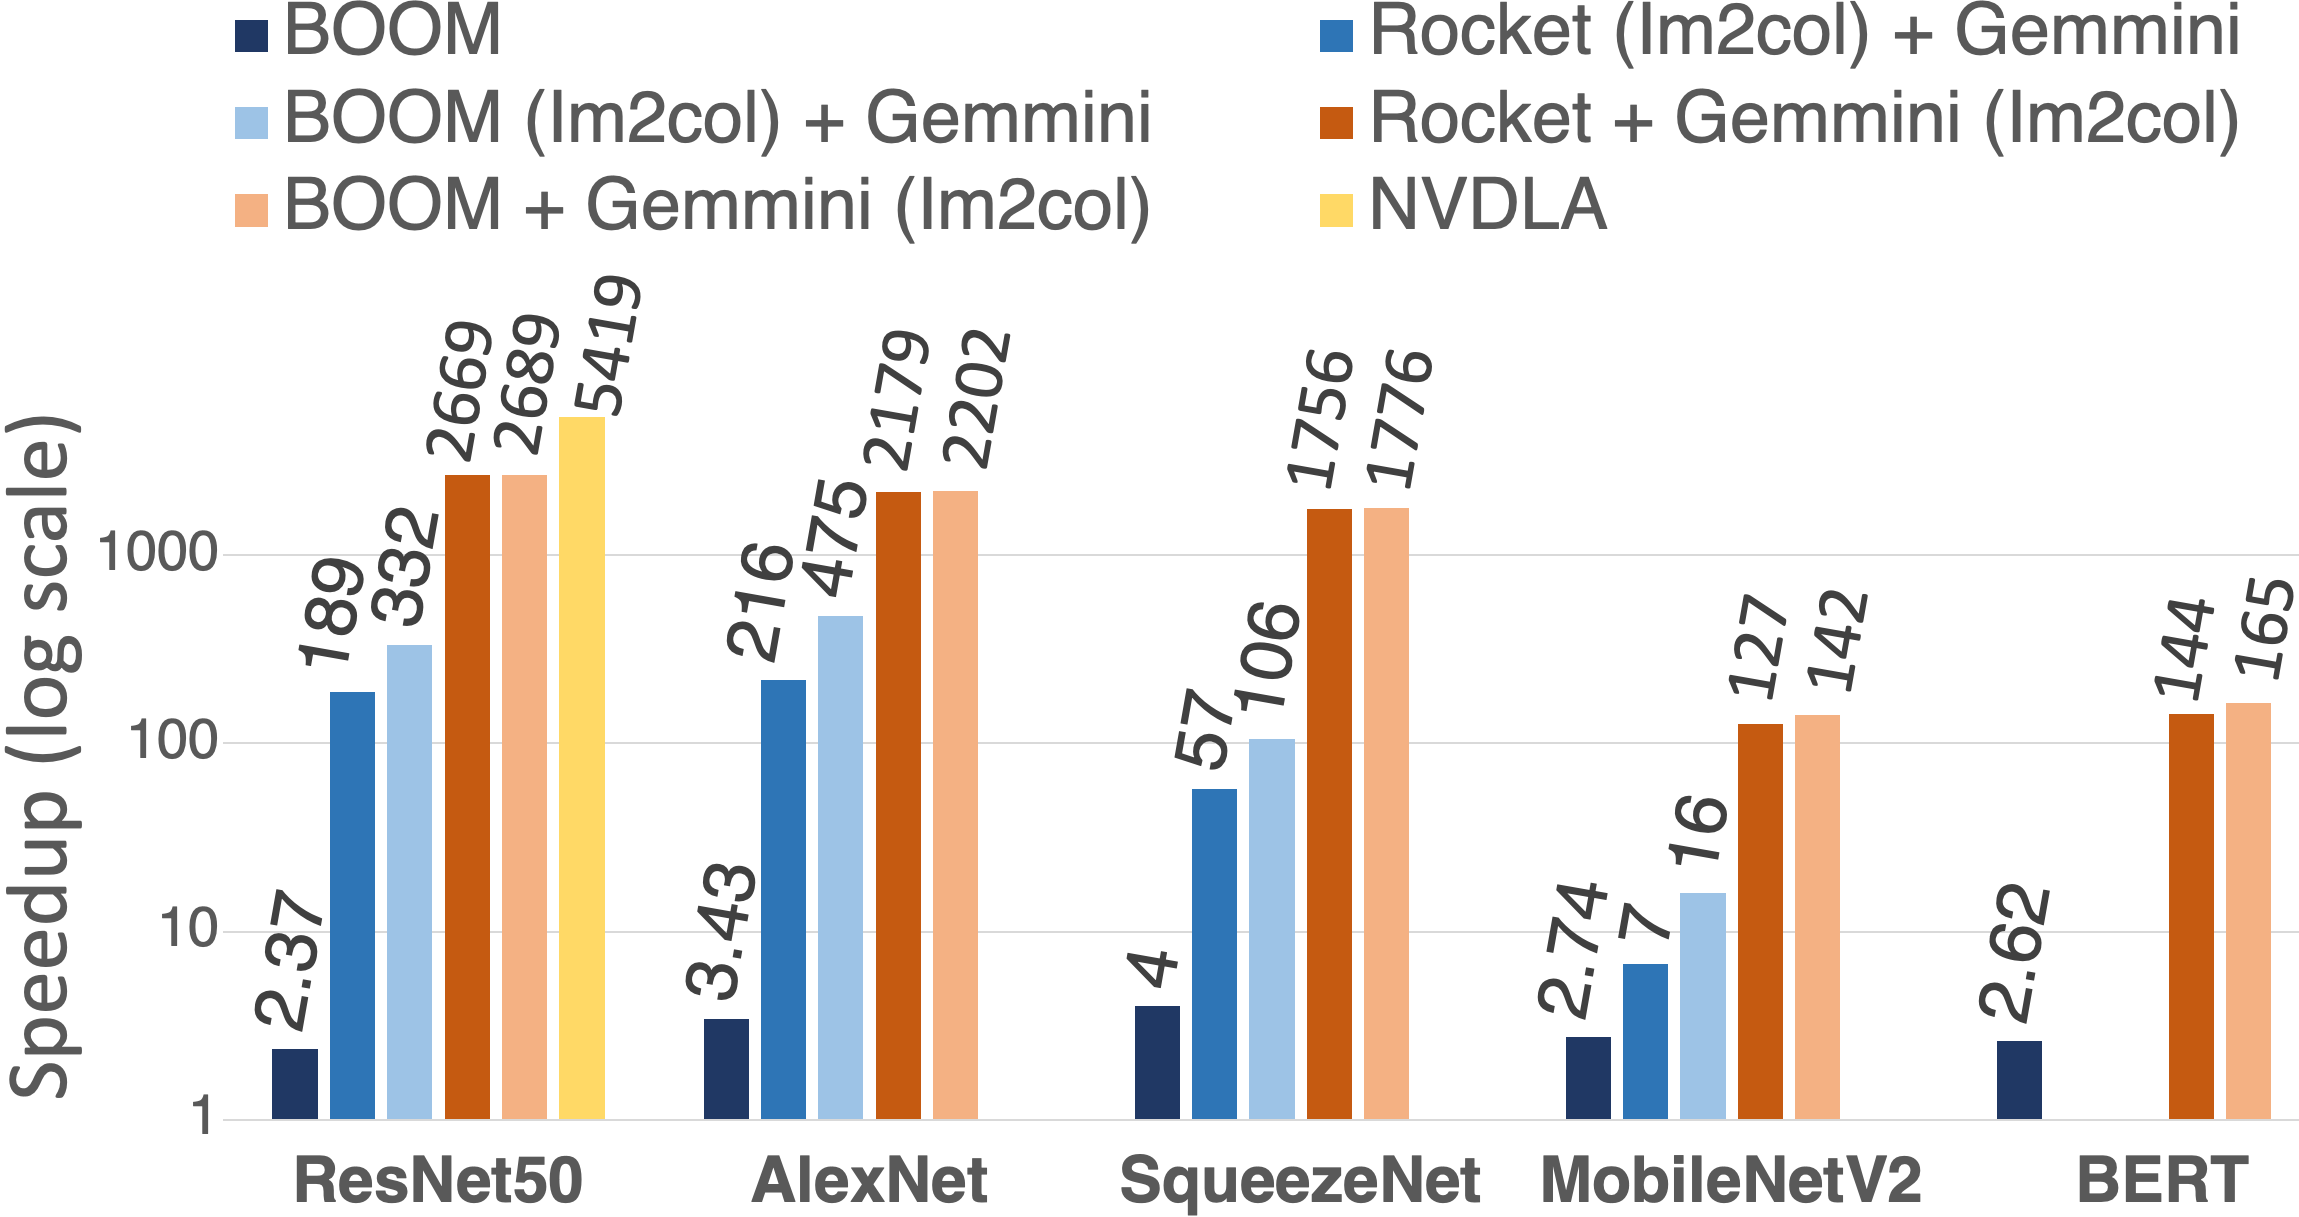
\includegraphics[width=\linewidth]{fig/perf-conv-new.png}
\caption{Speedup compared to an in-order CPU baseline. For CNNs, im2col was performed on either the CPU, or on the accelerator.}
\label{fig:perf-dnn}
\end{figure}

However, when the accelerator is equipped with an on-the-fly im2col unit, the choice of host CPU is far less important, because the CPU's computational burden is shifted further onto the accelerator. Adding a small amount of complexity to the accelerator allows us to reduce the area and complexity of the host CPU to a simple in-order core while preserving performance. Gemmini enables hardware designers to easily make these performance-efficiency tradeoffs.

With the on-the-fly im2col unit and a simple in-order Rocket CPU, Gemmini achieves 22.8 frames per second (FPS) for ResNet50 inference when running at 1 GHz, which is a 2,670x speedup over the in-order Rocket CPU and an 1,130x speedup over the out-of-order BOOM CPU. The accelerator also achieves 79.3 FPS on AlexNet. Some DNN models such as MobileNet are not efficiently mapped to spatial accelerators due to the low data reuse within the depthwise convolution layers. Therefore, Gemmini demonstrates only a 127x speedup compared to the Rocket host CPU on MobileNetV2, reaching 18.7 FPS at 1GHz.  On SqueezeNet, which was designed to be run efficiently on modern CPUs while conserving memory bandwidth, Gemmini still demonstrates a 1,760x speedup over the Rocket host CPU. Our results are comparable to other accelerators, such as NVDLA, when running with the same number of PEs as the configuration in Figure~\ref{tab:area-table}. When running language models such as BERT, Gemmini achieves a 144x improvement over the Rocket CPU.

% \textbf{Comparison to other accelerators:} Additionally, Figure~\mbox{\ref{fig:perf-dnn}} plots the performance of the state-of-the-art NVDLA accelerator~\mbox{\cite{nvdla-perf}},
% for those DNNs which NVDLA has published results for, as a comparison point with our Gemmini-generated accelerator. However, NVDLA's performance numbers came from an analytical model released by NVIDIA, rather than by actually running on an NVLDA instance comparable to our Gemmini-generated accelerator.
% Our results are comparable to other commercial accelerators which were tested with real hardware, such as the Kirin 970 NPU, which achieves 21.9 FPS on ResNet50, as compared to 23 FPS on our Gemmini-generated accelerator, with similar hardware resources~\mbox{\cite{kirin-perf}}.

% \begin{figure}[t]
% \centering
% 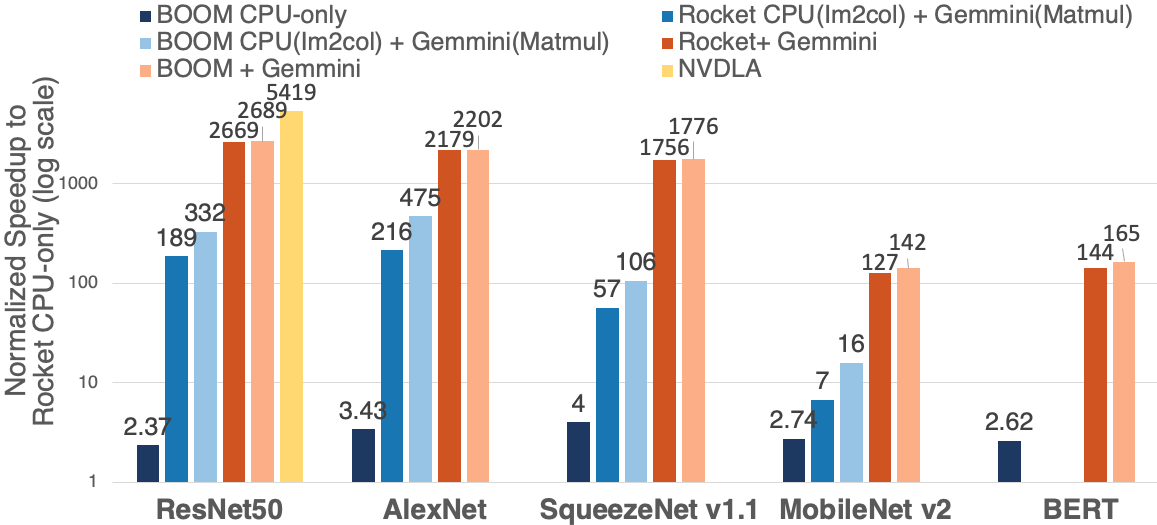
\includegraphics[width=0.95\columnwidth]{fig/perf-conv.png}
% \caption{Performance evaluation of Gemmini-generated accelerators with and without the im2col hardware module compared to a CPU baseline and NVDLA published performance. BERT has no convolutions, so im2col is not run as part of it.}
% \label{fig:perf-dnn}
% \vspace{-0.4cm}
% \end{figure}

% \textcolor{red}{Gemmini's does not reach NVDLA's performance is because the im2col block achieves low utilization on layers with few input channels, such as the RGB first layer input to our CNNs. Overlap between memory and compute instructions is also not as high as it could be due to a mismatch between the granularity of the memory and compute ISA instructions. This mismatch causes the Gemmini-generated accelerator's ROB to fill with instructions that cannot begin execution. Both these performance maladies are currently being rectified, and we expect our performance to improve closer towards NVDLA's baseline when they do.}


% According to \cite{nvdla-perf}, NVDLA reported both ResNet and AlexNet results by selecting the maximum value between DRAM communication cycles and MAC computation cycles for each layer and summing them. Furthermore, both numbers are made by numerical scaling from 2048 MAC / 512KB case.  This would mean they have assumed perfect overlap between data movement from/to DRAM and MAC computation, and perfect scaling, which might be optimistic. On the other hand, our results are from real end-to-end cycles, which captures any non-overlapped cycles between data movement and mesh operation as well as CPU code execution cycles, such as calculating tiling factors and iterating over nested loops by generated tiling factors.

%\footnote{AlexNet inference results for NVDLA are published only for the 2048 MAC / 512 KB configuration. Therefore, we divide that result by 8 in order to estimate against the equivalent Gemmini/NVDLA configuration}





